\documentclass[10pt]{beamer}
\usetheme{Boadilla} % My favorite!
\setbeamercovered{invisible}
% To remove the navigation symbols from 
% the bottom of slides%
\setbeamertemplate{navigation symbols}{} 
\setbeamertemplate{itemize items}[default]
\setbeamertemplate{enumerate items}[default]
\xdefinecolor{lavendar}{rgb}{0.2, 0.2, 0.72}
%
\usepackage{graphicx,epsfig}

%\usepackage{bm}         % For typesetting bold math (not \mathbold)
%\logo{\includegraphics[height=0.6cm]{yourlogo.eps}}
%

\newcommand{\be}{\begin{equation*}}
\newcommand{\ee}{\end{equation*}}
\newcommand{\ba}{\begin{eqnarray}}
\newcommand{\ea}{\end{eqnarray}}

\newcommand{\vso}{\vskip15pt}
\newcommand{\vst}{\vskip30pt}



\def\smallfrac#1#2{\hbox{${{#1}\over {#2}}$}}


\AtBeginSection[]
{
  \begin{frame}<beamer>{}
  \frametitle{Outline}
    \tableofcontents[currentsection]
  \end{frame}

}
\title[]{Reweighting NNPDFs}
\author{Nathan Hartland}
\institute
{
University of Edinburgh\\
%\includegraphics[height=2cm]{edinburghcrest.pdf}
\medskip
}
% \today will show current date. 
% Alternatively, you can specify a date.
%
\titlegraphic{\includegraphics[height=2cm]{edinburghcrest.pdf}}

\date{\today}


\begin{document}
\renewcommand{\inserttotalframenumber}{24}


\begin{frame}
\begin{centering}
\vskip20pt
\center{\huge\color{lavendar} \textbf{Reweighting NNPDFs}}
\vskip20pt
Nathan Hartland\\
\small{University of Edinburgh}
\vskip20pt
{\bf The NNPDF Collaboration:}\\
Richard~D.~Ball, Valerio~Bertone, Francesco~Cerutti,\\
Luigi~Del~Debbio, Stefano~Forte, Alberto~Guffanti, N.H,\\
Jos\'e~I.~Latorre, Juan~Rojo and Maria~Ubiali. 
\vskip40pt
Young Theorists' Forum 2011\\
Durham University\\
14th December 2011


\end{centering}

\end{frame}

\section{Parton distribution fitting}
\begin{frame}
\frametitle{Parton distributions for the LHC}
%\be \sigma = \Sum_{i,j} \int_0^1 dx_1dx_2 f_i(x_1,Q^2)f_j(x_2,Q^2)\sigma \left( x_1,x_2,Q^2 \right)  \ee

\be \sigma_X= \sum_{a,b} \int_0^1 dx_1dx_2 f_a(x_1,Q^2)f_b(x_2,Q^2)\sigma_{q_aq_b \to X} \left( x_1,x_2,Q^2 \right) \ee
\begin{itemize}
		\item<1-> Need to have a reliable determination of PDFs for LHC physics!
		\item<1-> For many EW processes PDF uncertainty dominates - good uncertainty analysis is crucial.

\end{itemize}
\vskip15pt
\center{PDF $x$-dependence determined by a fit to experimental data.}
\center{PDF behaviour in $Q^2$: DGLAP Evolution.}

\vskip15pt
\begin{block} {Fitting groups}

\begin{columns}
  \begin{column}{0.5\textwidth}
\begin{itemize}
  \setlength{\itemindent}{1em}

		\item<1->MSTW
		\item<1->CTEQ
		\item<1->NNPDF
	\end{itemize} 

	
	 \end{column}

  \begin{column}{0.5\textwidth}
\begin{itemize}
		\item<1->HERAPDF
		\item<1->ABKM
		\item<1->GJR
	\end{itemize}  \end{column}
\end{columns}
\end{block}


\end{frame}


\begin{frame}
\frametitle{Parton distributions for the LHC}
\begin{figure}[b!]
    \begin{center}
      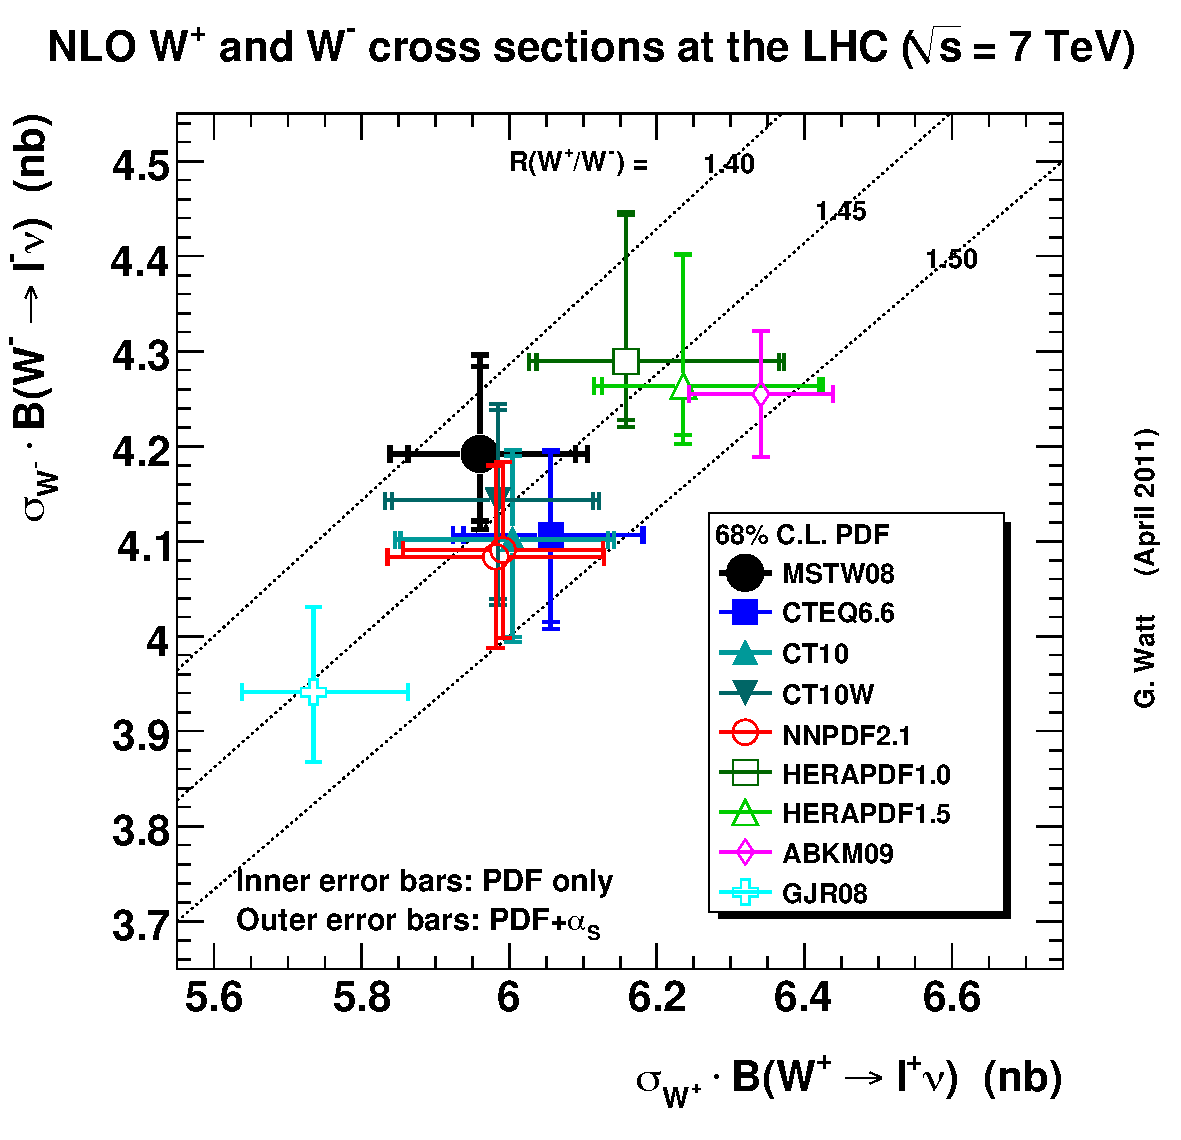
\includegraphics[width=0.55\textwidth]{w+w-lhc7nlo68err.eps}
    \end{center}
\end{figure}
{ \centering \small \color{blue} G. Watt [arXiv:1106.5788 [hep-ph]]}\\
Standard Candles: Generally good agreement between global PDF fits.
\end{frame}
\begin{frame}
\frametitle{Parton distributions for the LHC}
\begin{figure}[b!]
    \begin{center}
            \includegraphics[width=0.85\textwidth]{ratiogglumi1_68cl.eps}
    \end{center}
\end{figure}
{ \centering \small \color{blue} G. Watt [arXiv:1106.5788 [hep-ph]]}\\
Discrepancies: Use envelope of PDF uncertainties.
\end{frame}


\begin{frame}
\frametitle{Parton distribution fitting - the standard approach}
Choose a functional form for your PDFs.
\begin{block} {\centering Typical Parametrisations}
\begin{itemize}
		\item<1->MSTW08     \be f(x,Q_0^2) \sim ax^{b}(1-x)^{c}(1+d\sqrt{x}+e x),\ee
		\item<1->CT10    \be f(x,Q_0^2) \sim ax^b(1-x)^c \exp{(dx + ex^2 + f\sqrt{x})}.\ee
	\end{itemize}
\end{block}
	\vskip15pt
MSTW08, CT10 fits have in total ~20 - 26 free parameters.
\vskip10pt
Evolve to the required scale, and compute physical observables.\\
Minimise some measure of fit quality w.r.t. the data.
	\be \chi^2(a)=\frac{1}{N_{dat}}\sum_{i,j=1}^{N_{dat}}(D_i-T_i(a))(\sigma_{ij})^{-1}(D_j-T_j(a)).\ee

\end{frame}


\begin{frame}
\frametitle{Standard approach to parton fitting - uncertainties}
How to propagate uncertainties from the experimental data to the PDFs?
\underline{Standard Approach}: Linear propagation of uncertainties by Hessian Method.
\begin{itemize}
		\item<1->For a set of fit parameters $\{ a\} $ define a tolerance in $\chi^2$:
		\be \Delta\chi^2(a) \equiv \chi^2(a) - \chi^2(a^\mathrm{min}) = \sum^n_{i,j=1}H_{ij}(a_i-a_i^\mathrm{min})(a_j - a_j^\mathrm{min}). \ee
		\item<1-> Determine PDFs on surface of constant $\Delta\chi^2=T$ in parameter space.
		\begin{itemize}
			\item<1-> Numerical difficulties: Need to use rescaled eigenvectors of $H$.
		\end{itemize}
		\item<1-> Obtain $2n$ PDF sets $S_i^\pm$, where $n$ is the number of free parameters in the fit. \vso
		\item<1-> Uncertainty in an observable $\mathcal{O}$ given by:
		\be \mathrm{Var}[\mathcal{O}] = \frac{1}{2}\sum_{i=0}^n (\mathcal{O}[S_i^+] - \mathcal{O}[S_i^-] )^2.\ee
\end{itemize}

\end{frame}

\begin{frame}
\frametitle{Difficulties with the standard approach}
\begin{itemize}
\item<1-> Determining correct tolerance $T$. 
\begin{itemize}
\item<1-> Ideal value $T=1$ leads to unrealistically small errors.
\item<1-> CTEQ choice $T \sim 100$
\item<1-> MSTW - dynamical procedure: $T \sim 5-20$.
\end{itemize}
\vst
\item<1->Parametrisation Bias
\begin{itemize}
\item<1-> Choice of functional form may lead to biased fit.
\item<1-> Inflexible parameterisation may artificially constrain PDF errors.
\item<1-> PDF errors may \emph{increase} when data is added due to the need to add more parameters.  
\end{itemize}

\end{itemize}
\vst	
	
	\center{Can we do things differently?}

\end{frame}


\section{The NNPDF methodology}

\begin{frame}
\frametitle{NNPDF parameterisation}
\underline{Idea}: Use artificial neural networks to parameterise the PDFs.
\begin{itemize}
\item<1-> Neural nets: just another functional form.
\item<1-> Each neural net in the NNPDF fit - 37 free parameters.
\end{itemize}
\vso
Robust, massively redundant parameterization:
\begin{itemize}
\item<1-> An NNPDF parton fit has in total 259 fit parameters.
\item<1-> Neural nets are extremely flexible, unbiased function approximators.
\end{itemize}
\vso

\hfill\begin{minipage}{6cm}
\begin{block}
{ \centering NNPDF functional form}
\be f(x)=(1-x)^{a}x^{-b} \mathrm{NN}(x). \ee
\end{block}
\end{minipage}\hfill{}


\end{frame}

\begin{frame}
\frametitle{Monte Carlo uncertainty determination}
\begin{itemize}
\item<1->Form an ensemble of $N$ artificial data 'replicas' by importance sampling the original data set.
\\
\item<1->The ensemble of artificial data replicas forms a representation of the probability distribution in data.
\\
\item<1->Perform a separate fit to each data replica, obtain an ensemble of PDF replicas.
\\
\end{itemize}
 \begin{figure}[b!]
    \begin{center}
      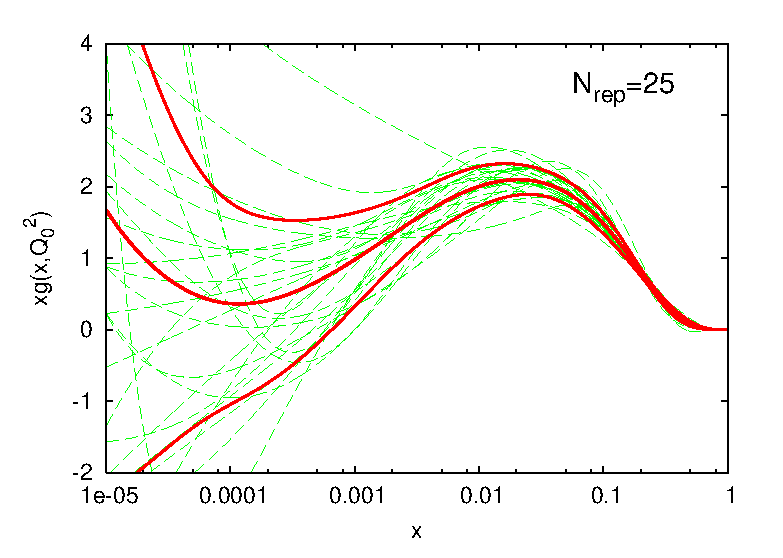
\includegraphics[width=0.45\textwidth]{glureplicas25.eps}
      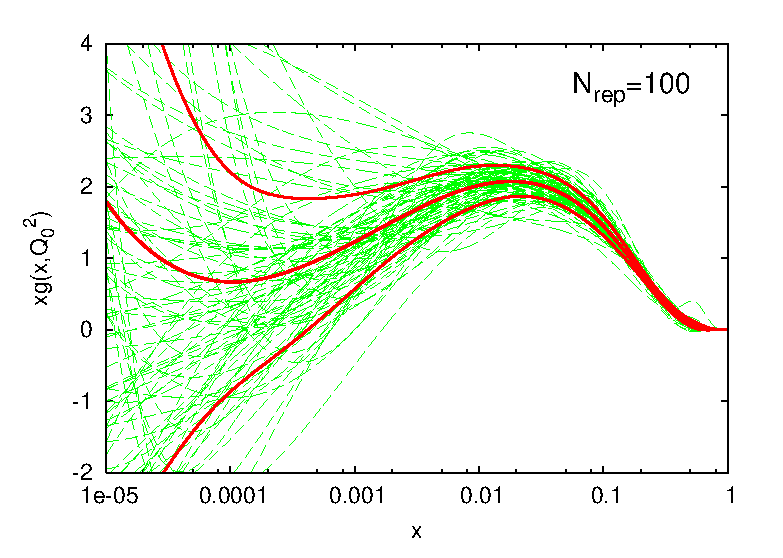
\includegraphics[width=0.45\textwidth]{glureplicas100.eps}
    \end{center}
    \vskip-0.5cm
    \label{fig:pdf-jets}
\end{figure}


\end{frame}

\begin{frame}
\frametitle{NNPDF User Guide}

\begin{block}
{Central value predictions}
		\be \langle\mathcal{O}\rangle=\smallfrac{1}{N}\,\sum_{k=1}^{N}\mathcal{O}[f_k]\, .\ee
\end{block}
\vso
\begin{block}
{Uncertainties }
		\be {\mathrm{Var}}[\mathcal{O}]=\smallfrac{1}{N}\,\sum_{k=1}^{N}(\mathcal{O}[f_k] -  \langle\mathcal{O}\rangle )^2 .\ee
\end{block}
\vso
\center{Uncertainties in the PDFs faithfully represent the experimental data. \\No tolerance criterion is required.}

\end{frame}

%\begin{frame}
%\frametitle{The NNPDF Methodology }
%
%\begin{itemize}
%		\item<1-> Neural Network parametrization of PDFs \\
%		{ \color{blue} Redundant parametrization for an unbiased fit.}\vso
%		\item<1-> Monte Carlo uncertainty determination.\\
%		{ \color{blue}Faithful representation of the experimental uncertainties.}\vso
%		\item<1-> Genetic Algorithm for minimisation. \\
%		{ \color{blue}Efficient minimisation in a large parameter space.}\vso
%		\item<1-> Dynamical fit stopping by cross-validation. \\
%		{ \color{blue} Preventing overfitting.}
%		
%	\end{itemize}
%	
%	
%\end{frame}




\section{The reweighting method}

\begin{frame}
\frametitle{Including new experimental data}
How can we add new data to an existing parton set?

\begin{itemize}
		\item<1-> Full Refit\\
		Time consuming, can only be done by the fitting collaboration.
		\item<1-> Reweight existing Monte Carlo parton set. {\small \color{blue} Giele, Keller [hep-ph/9803393] }\\
\end{itemize}
If the new data is statistically independent of the data in the prior set:
\be
\mathcal{P}_{\rm new}(f)
= \mathcal{N}_{\chi}\mathcal{P}(\chi^2|f)\;\mathcal{P}_{\rm old}(f),
\ee
		\be \langle\mathcal{O}\rangle_{\mathrm {new}}=\int \mathcal{O}[f] \, \mathcal{P}_{ \mathrm {new}}(f)\,Df=\smallfrac{1}{N}\,\sum_{k=1}^{N}w_k\mathcal{O}[f_k].\,  \ee
Weights determined by statistical inference
\be w_k =\mathcal{N}_\chi\mathcal{P}(\chi^2|f_k) = 
\frac{(\chi^{2}_k)^{(n-1)/2} 
e^{-\frac{1}{2}\chi^{2}_k}}
{\smallfrac{1}{N}\sum_{k=1}^{N}(\chi^{2}_k)^{(n-1)/2}
e^{-\frac{1}{2}\chi^{2}_k}}\, .\ee
\center{ \small  R.~D.~Ball {\it et al.} Nucl.\ Phys.\ B {\bf 849} 112  [arXiv:1012.0836]. }

\end{frame}



\begin{frame}
\frametitle{Verification of the reweighting method}
\begin{itemize}
		\item<1-> Produce a 1000 replica NNPDF fit to DIS and DY data only.
		\begin{itemize}
		\item<1-> NNPDF2.0(DIS+DY)
		\end{itemize}
		\item<1-> Reweight this set with Tevatron inclusive jet data.
		\item<1-> Compare reweighted set to the full fit.
				\begin{itemize}
		\item<1-> NNPDF2.0
		\end{itemize}
\end{itemize}
 \begin{figure}[b!]
    \begin{center}
      \includegraphics[width=0.50\textwidth]{jets-t0-xg_Q2_2_lin.eps}
      \includegraphics[width=0.50\textwidth]{jets-t0-abserror-xg_Q2_2_lin.eps}
    \end{center}
    \vskip-0.5cm

\end{figure} \vso

\center{Distributions equivalent up to statistical fluctuations.}

\end{frame}

\begin{frame}
\frametitle{Error rescaling parameter}
Useful tool for analysing experimental uncertainties.
\begin{itemize}
		\item<1-> Rescale uncertainties by a factor $\alpha$.
		\item<1-> Compute a new weight $w_k(\alpha)$ with these uncertainties.
		\item<1-> Average over all replicas $\to$ probability of rescaling uncertainties by $\alpha$.
\end{itemize}


\begin{columns}
  \begin{column}{0.5\textwidth}
  \begin{block}{}
\be \chi^2_{k,\alpha} = \chi^2_k/\alpha^2, \ee
\be w_k(\alpha) = (\chi^2_{k,\alpha})^{(n-1)/2}\mathrm{e}^{-\chi^2_{k,\alpha}/2,}\ee
\be \mathcal{P}(\alpha)\propto \smallfrac{1}{\alpha}\sum_{k=1}^N w_k(\alpha).\ee
\end{block}
  \end{column}
  
    \begin{column}{0.5\textwidth}
    \center{ \small Tevatron Jets $\mathcal{P}(\alpha)$}
 \begin{figure}[b!]
    \begin{center}
      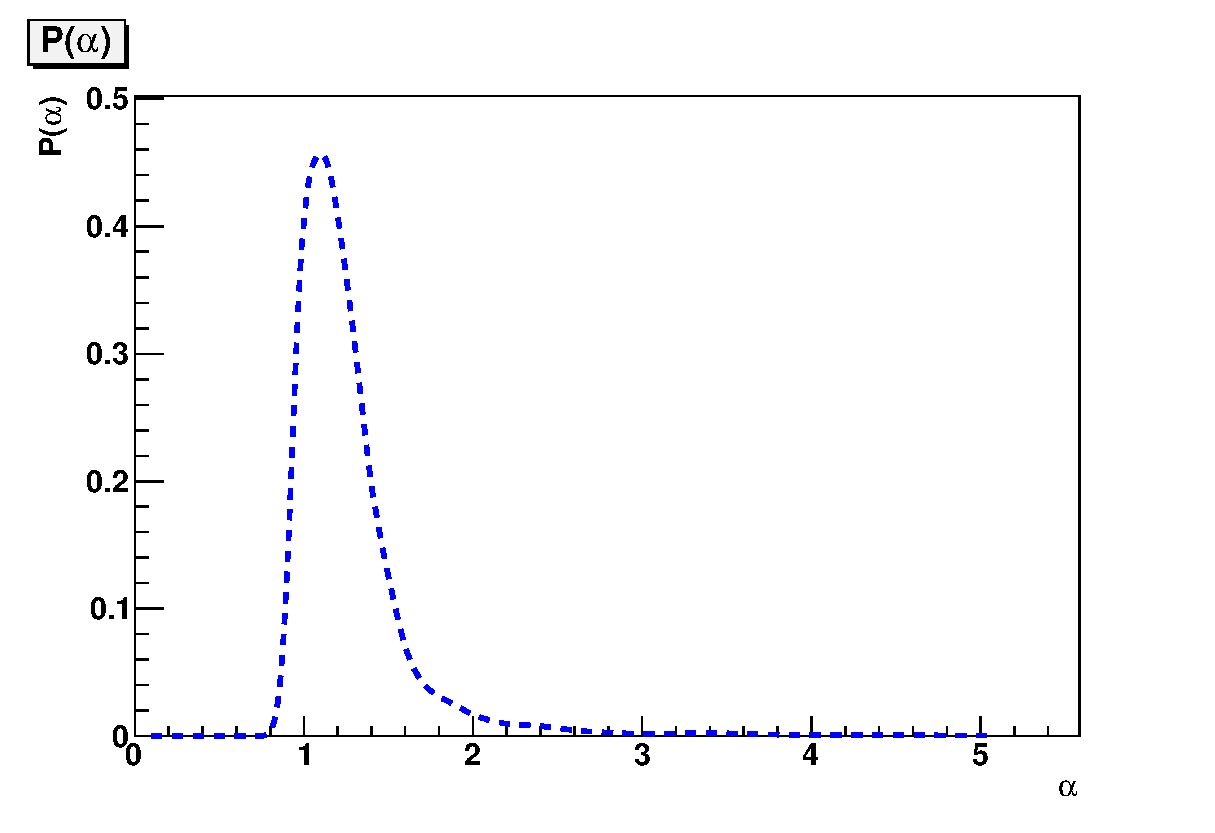
\includegraphics[width=1\textwidth]{palpha-jets-t0.eps}
    \end{center}
\end{figure}

  \end{column}  
  \end{columns}

\begin{figure}[b!]
    \begin{center}
    \end{center}
    \vskip-0.5cm

\end{figure}



\end{frame}


\begin{frame}
\frametitle{Ensemble Efficiency}

   \begin{itemize}
		\item<1-> Prior set: maximally efficient representation of probability distribution.
		\item<1-> Reweighted set: loss of efficiency due to very small weights.
		\item<1-> Many replicas no longer contribute to the ensemble.
\end{itemize}

\center{Loss of information quantified by the Shannon entropy:}
  \be N_{\textrm{ eff}} \equiv \exp \left(\frac{1}{N_{\mathrm{rep}}}\sum_{k=1}^{N_{\mathrm{rep}}}w_k\ln(N_{\mathrm{rep}}/w_k)\right)\ee
\begin{columns}
  \begin{column}{0.45\textwidth}
 \begin{figure}[b!]
    \begin{center}
      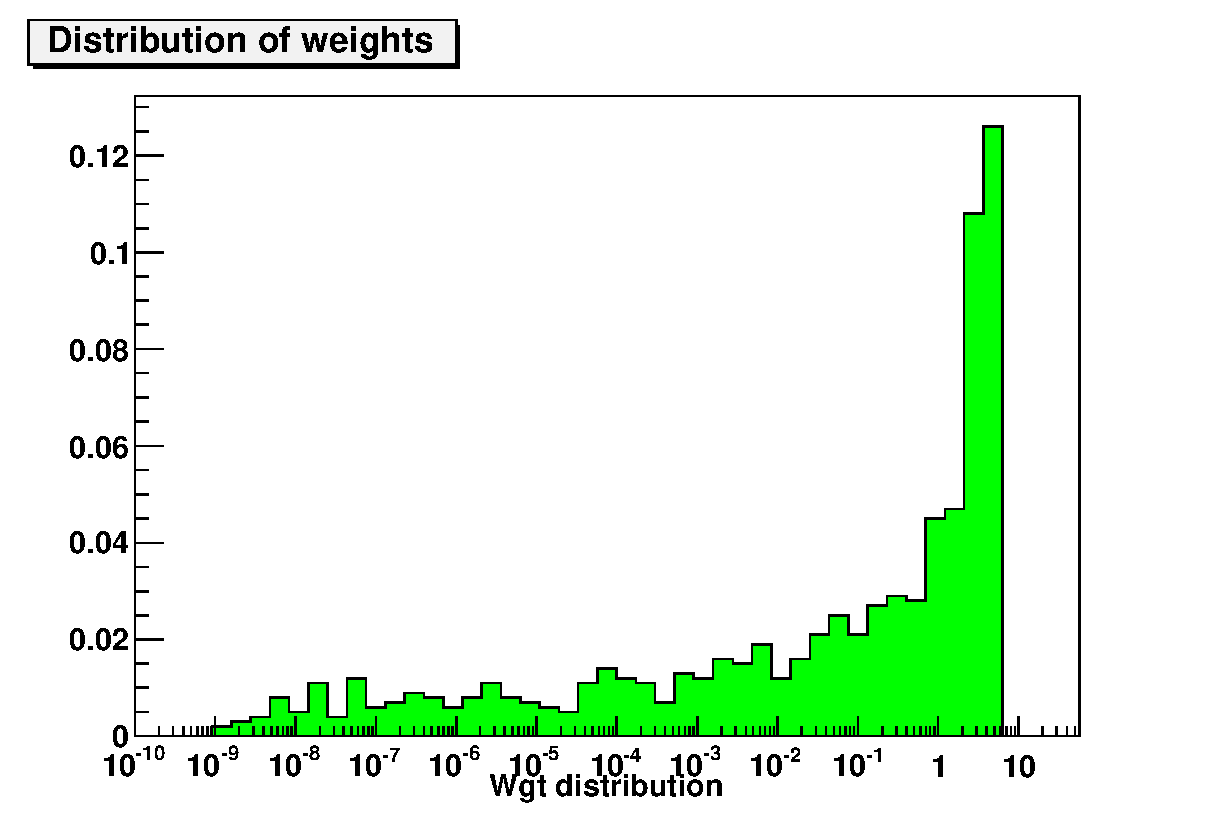
\includegraphics[width=0.85\textwidth]{wgt-dist-jets-t0.eps}
    \end{center}
\end{figure}

  \end{column}

  \begin{column}{0.55\textwidth}
  A very low $N_{\textrm{ eff}}$ means data is either:
 \begin{itemize}
		\item<1-> Very constraining
		\item<1-> Inconsistent with prior
\end{itemize}
\vskip10pt
Tevatron Jet reweighting: $N_{\textrm{ eff}}=334.5$.
     \end{column}
\end{columns}
\end{frame}



\begin{frame}
\frametitle{Producing unweighted PDFs}
  \small \underline{Aim}: to produce a set of PDFs without weights, but equivalent to a reweighted set. 
\vso
\underline{Method}: Deterministically sample with replacement weighted replica distribution.
\begin{itemize}
		\item<1-> Form new set with $N_{rep}^\prime$ replicas.
		\item<1-> Replicas with small weights not included in new set.
		\item<1-> Replicas with very high weights counted repeatedly.
\end{itemize}
\vso
\center{\textbf{Weights in reweighted set represented as multiplicities in unweighted set.}}
\vso
\center{Allows us to perform further checks on the consistency of the procedure.}\\
\end{frame}

\begin{frame}
\frametitle{Consistency check - Multiple Reweighting}
Reweighting with two data sets can be performed by:
\begin{itemize}
		\item<1-> Reweighting with the combined dataset.
		\item<1-> Reweighting with one data set, and then the other.
\end{itemize}
\vso
To check consistency of reweighting, need to demonstrate
\be    \hat{U}\hat{R}_{12} = \hat{U}\hat{R_2}\hat{U} \hat{R}_1 = \hat{U}\hat{R}_1 \hat{U}\hat{R}_2. \ee
\vso
\underline{Test Case}: We reweight a DIS only fit (NNPDF2.1 DIS) with
\begin{itemize}
		\item<1-> E605 Fixed target Drell-Yan data.
		\item<1-> Tevatron Run II inclusive jet data.
\end{itemize}

\begin{table}[t]
  \centering
  \begin{tabular}[c]{|c|c|c|c|}
    \hline
    & Jets & E605 & Jets +E605 \\
    \hline
    Data points & 186 & 119 & 305 \\
    \hline
    $N_{\rm eff}$ & 627.1 & 59.5 & 63.7\\
    \hline
  \end{tabular}
\end{table}

\end{frame}

\begin{frame}
\frametitle{Consistency check - Multiple Reweighting}
\begin{figure}
  \epsfig{width=0.9\textwidth,figure=e605-jets_xg_lin_zoom_rel.eps}
\end{figure}
\end{frame}

\begin{frame}
\frametitle{Application: NNPDF2.2 Parton Set .}
\center{\textbf{First global PDF set including data from the LHC}}\\
New data added by reweighting NNPDF2.1 Fit: $W$ leptonic charge asymmetry.
\center{\small  R.~D.~Ball {\it et al}, Nucl.\ Phys.\ B {\bf 855} 608 {\color{blue} [arXiv:1108.1758] }.}\vso
Defined in terms of $W^{\pm}\to l^\pm\nu_l $ differential cross-sections $d\sigma_{l^\pm}/d\eta_l$
\be 
  A^l_W=\frac{d\sigma_{l^{+}}/d\eta_{l}-d\sigma_{l^{-}}/d\eta_{l}}
  {d\sigma_{l^{+}}/d\eta_{l}+d\sigma_{l^{-}}/d\eta_{l}}, 
\ee


\begin{itemize}
		\item<1-> ATLAS $\mu$ charge asymmetry. \hspace*{\fill {  \color{blue} [arXiv:1103.2929]}}
		\item<1-> CMS $e+\mu$ charge asymmetry. \hspace*{\fill { \color{blue}  [arXiv:1103.3470] }}
		\item<1-> D0 $e+\mu$ charge asymmetry. \hspace*{\fill { \color{blue} [arXiv:0709.4254]}}
\end{itemize}

\begin{figure}[htb]
  \begin{center}
    \epsfig{width=0.32\textwidth,figure=atlas.eps}
    \epsfig{width=0.32\textwidth,figure=cms_el_25pt.eps}
    \epsfig{width=0.32\textwidth,figure=cms_mu_25pt.eps}
  \end{center}
  \end{figure}

\end{frame}


\begin{frame}
\frametitle{Fit quality}
\begin{columns}
  \begin{column}{0.5\textwidth}
    \centering
NNPDF2.1 LHC
 \begin{figure}[h!]
  \centering
  \epsfig{width=0.9\textwidth,figure=palpha-lhc25.eps}
\end{figure}
     \end{column}
       \begin{column}{0.5\textwidth}
           \centering
NNPDF2.2
 \begin{figure}[h!]
  \centering
  \epsfig{width=0.9\textwidth,figure=palpha-tev+lhc25.eps}
\end{figure}
          \end{column}

\end{columns}

\begin{table}
  \begin{center}
    \begin{tabular}{|c|c|c|c|c|}
      \hline 
      Experiment & $N_{\mathrm{dat}} $ & NNPDF2.1 & NNPDF2.1 LHC & NNPDF2.2 \\
      \hline
      \hline
      \hline
      ATLASmuASY &   11 & [0.77]  &  0.97    &  1.07  \\
      \hline
      CMSeASY    &   6 &  [1.83]  &  1.23    &  1.08  \\
      \hline
      CMSmuASY   &   6 &  [1.24]  &  0.63    &  0.56  \\
      \hline
      D0eASY     &   12 & [4.39]  &  [3.46]  &  1.38  \\
      \hline
      D0muASY    &   10 & [1.48]  &  [1.17]  &  0.35  \\
      \hline
      \hline
      Full Dataset     &      &  1.165 &  1.158 &  1.157 \\
      \hline
    \end{tabular}
\end{center}
\end{table}

\end{frame}


\begin{frame}
\frametitle{First LHC constraints on parton distributions}
\begin{figure}[h!]
  \centering
  \epsfig{width=0.44\textwidth,figure=xu-nnpdf22.eps}
  \epsfig{width=0.44\textwidth,figure=xubar-nnpdf22.eps}
  \epsfig{width=0.44\textwidth,figure=xd-nnpdf22.eps}
  \epsfig{width=0.44\textwidth,figure=xdbar-nnpdf22.eps}
\end{figure}
\end{frame}
 
\begin{frame}
\frametitle{Summary}
\begin{itemize}
\item<1-> NNPDF Parton Sets
\begin{itemize}
		\item<1-> Neural Network parametrisation of PDFs. \\
		{ \color{blue} Redundant parametrisation for an unbiased fit.}
		\item<1-> Monte Carlo uncertainty determination.\\
		{ \color{blue}Faithful representation of the experimental uncertainties.}\vso
		\end{itemize}
\item<1-> Bayesian Reweighting
\begin{itemize}
		\item<1-> Powerful technique for including new data into existing parton fits. \\
		{ \color{blue} Fast assessment of data impact.}\vso
		\end{itemize}
\item<1-> NNPDF2.2
\begin{itemize}
		\item<1-> First PDF set including LHC data. \\
		{ \color{blue} W lepton asymmetry data provides small constraint on light quark PDFs.}\vso
		\end{itemize}
\end{itemize}
\centerline{NNPDF2.1 and NNPDF2.2 PDF Sets available through LHAPDF}


\end{frame}
%
%\begin{frame}
%    \begin{center}
%      BACKUPS
%    \end{center}
%\end{frame}
%
%
%
%\begin{frame}
%\small
%\frametitle{Special features of NNPDF approach}
%\textbf{Minimisation by genetic algorithms}\\
%\underline{Problem}: Very large parameter space, $\chi2$ highly nonlocal. \begin{itemize}
%\item<1-> Minimisation is challenging.
%\end{itemize}\underline{Solution}: Genetic Algorithms (GA)
%\begin{itemize}
%\item<1-> Generate mutations of fit parameters.
%\item<1-> Select those mutations that minimise figure of merit.
%\end{itemize}
%\vskip10pt
%\textbf{ Dynamical fit stopping by cross-validation}\\
%\underline{Problem}:  extremely flexible parameterisations are prone to \emph{overfitting}.
%\\
%\begin{itemize}
%\item<1->Fit has so many parameters, the minimum $\chi^2$ corresponds to a fit not only to
%the data, but also statistical noise.
%\end{itemize}
%\underline{Solution}:  dynamical stopping by \emph{Cross Validation}.
%\begin{itemize}
%\item<1-> Split the dataset into a training set and a validation set.
%\item<1-> Use the training set for minimisation, monitor the $\chi^2$ to the validation set.
%\item<1-> Stop the fit when the $\chi^2$ to the validation set starts to increase while
%the $\chi^2$ to training set is still decreasing.
%
%\end{itemize}
%
%
%
%\end{frame}
%
%\begin{frame}
%\frametitle{Cross Validation}
% \begin{figure}[b!]
%    \begin{center}
%      \includegraphics[width=0.9\textwidth]{chi2ite-1004-NMC-pd.eps}
%    \end{center}
%\end{figure}
%\end{frame}
%
%\begin{frame}
%\frametitle{Unweighting procedure}
%\begin{columns}
%  \begin{column}{0.5\textwidth}
%\begin{figure}
%  \epsfig{width=0.7\textwidth,figure=unwplot-1.eps,angle=-90}\\
%\end{figure}
%  \end{column}
%  \begin{column}{0.5\textwidth}
%\begin{figure}
%  \epsfig{width=0.7\textwidth,figure=unwplot-2.eps,angle=-90}
%\end{figure}
%  \end{column}
%\end{columns}
%\end{frame}
%

% End of slides
\end{document} 